% Copyright (C) 2022 by Maxime CHUPIN
% Modificado para o template do TCC

\documentclass[10pt,aspectratio=169,brazil]{beamer}
% \usepackage[charter]{mathdesign} % Comentado para usar a fonte matemática padrão do LaTeX
\usepackage{babel}
\usepackage{tcolorbox}
\usepackage{biblatex}
\usepackage{cleveref}
\usepackage{amsmath, amssymb}
\usepackage{physics}
\usepackage{bm}

\usetheme{Amurmaple}

\title[SciML em Boussinesq]{Inteligência Artificial na Solução Numérica de Equações Diferenciais Parciais Não Lineares}
\author[Samuel Kutz Paranhos]{Samuel Kutz Paranhos}
\subtitle{Aplicação de PINN, FNO e PINO no Sistema de Boussinesq}
\institute[UFPR]{Universidade Federal do Paraná (UFPR) \\ Laboratório de Dinâmica dos Fluidos Computacional (LabFluid)}
\date{Dezembro, 2025}

% Logo na página de título
\titlegraphic{
\includegraphics[width=4cm]{imgs/LabFluidLogoh.png}}


\bibliography{bibfile.bib}
\usefonttheme{serif}

\begin{document}

\maketitle

\sepframe[title={Sumário}]
\begin{frame}{Sumário}
\tableofcontents
\end{frame}

\section{Introdução}

\begin{frame}{Introdução e Motivação}

\end{frame}

\begin{frame}{Objetivos da Pesquisa}

\end{frame}
\section{O Sistema de Boussinesq}

\begin{frame}{Sistema de Boussinesq Parametrizado}

\end{frame} 
\section{Métodos de Scientific Machine Learning}

\begin{frame}{Physics-Informed Neural Networks (PINNs)}

\end{frame}

\begin{frame}{Fourier Neural Operators (FNO)}

\end{frame}


\begin{frame}{Physics-Informed Neural Operator (PINO)}

\end{frame}
\section{Metodologia Experimental}

\begin{frame}{Configurações dos Experimentos e Geração dos Dados}

\end{frame}
\section{Resultados e Discussão (Painéis)}

\begin{frame}{Resultados de Performance - Fourier Neural Operator}

\end{frame}

\begin{frame}{Resultados de Performance - Physics-Informed Neural Operator (PINO)}

\end{frame}

\begin{frame}{Treinamento Iterativo: FNO e PINO}

\end{frame}

\begin{frame}{Resultados e Treinamento - PINN}

\end{frame}
\section{Conclusões}

\begin{frame}{Principais Resultados}

\end{frame}


\begin{frame}[plain]
    \begin{center}
        \vspace*{1.5cm}
        \Huge \textbf{\textcolor{AmurmapleBlue}{Obrigado!}}
        \vspace*{1.5cm}
        
        \begin{figure}[!h]
            \centering
            \begin{minipage}{0.3\textwidth}
                \centering
                
\includegraphics[height=1.5cm]{imgs/ufpr_logo.jpg}
            \end{minipage}%
            \begin{minipage}{0.3\textwidth}
                \centering
                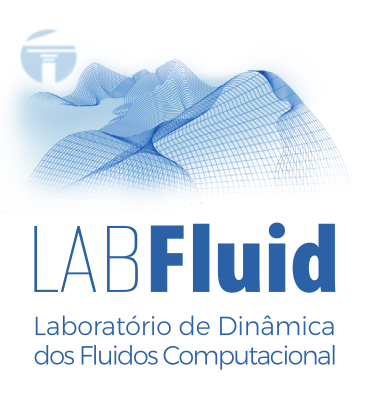
\includegraphics[height=1.5cm]{imgs/LabFluidLogo.png}
            \end{minipage}%
            \begin{minipage}{0.3\textwidth}
                \centering
                
\includegraphics[height=1.5cm]{imgs/CNPq.png}
            \end{minipage}
        \end{figure}
    \end{center}    
\end{frame}

\end{document}